\documentclass[main.tex]{subfiles}

\begin{document}
\sloppy

\vspace{1.0cm}

\section{Nuovo approccio all'interpolazione}\label{sec:Interpolation}
\lstset{language=UEcpp}
L'oggetto interpolazione si occupa di emulare lo spostamento di un vero motore nella realtà. Ad una interpolazione è possibile impostare un target, ed il valore fornito in output da questo oggetto verrà modificato ad ogni tick seguendo una velocità che accelera, rimane costante e decelera, fino a raggiungere il suddetto target.

L'oggetto interpolazione originale era implementato attraverso varie formule matematiche di derivate e integrali, che però erano difficile da modificare se necessario, non erano documentate, ma soprattutto non funzionavano: come già accennato nell'introduzione, molte volte il valore dell'interpolazione non convergeva verso il target continuando ad alternarsi intorno ad esso, oppure lo spostamento era molto lento. Inoltre non era possibile specificare davvero la velocità in secondi con il quale doveva accelerare o arrivare a destinazione, cosa invece richiesta da GDTF.\newline

In questo capitolo viene trattato come è stato completamente re-implementato l'algoritmo di interpolazione in una maniera più standard. Dopo essermi confrontato con le persone che lavorano al firmware dei fari nel reparto R\&D di ClayPaky, ho anche avuto conferma che la mia implementazione è molto vicina a quella presente nei fari veri.

\subsection{Prima implementazione}\label{subsec:4_trafficImplementation}
Un problema simile a questo era già stato riscontrato nell'implementazione di un progetto per l'esame di \say{Metodologie di Programmazione} \cite{TrafficGame}: Il progetto consisteva in un videogioco in cui erano presenti delle macchine che dovevano muoversi senza scontrarsi con quelle davanti. Ogni macchina doveva avere un movimento realistico, quindi, partendo da ferma, doveva accelerare e, per fermarsi, doveva decelerare. La scrittura di questo algoritmo è partita da quello presente in quel progetto. Le uniche due differenze consistono che nel progetto d'esame le macchine potevano andare solamente \say{avanti} ed il tempo tra un frame e l'altro del videogioco era constante, mentre su Unreal Engine è variabile. Quest'ultima differenza ci porta a dover mettere in atto numerose modifiche esposte nei capitoli successivi.\newline

Internamente la nostra velocità è salvata come \lstinline{float currentSpeed;} che dovrà rimanere nel range [0, 1]. All'interno dell'oggetto interpolazione verranno salvati due parametri:
\begin{itemize}
    \item \lstinline{acceleration}: quanta velocità perdiamo o guadagniamo ogni secondo, espressa come valore normalizzato tra [0, 1].
    \item \lstinline{maxPhysicalSpeed}: quanta distanza fisica viene percorsa ogni secondo mentre stiamo alla velocità massima (da qui in avanti chiamata \say{maxSpeed}).
\end{itemize}
\begin{figure}[H]
    \centering
    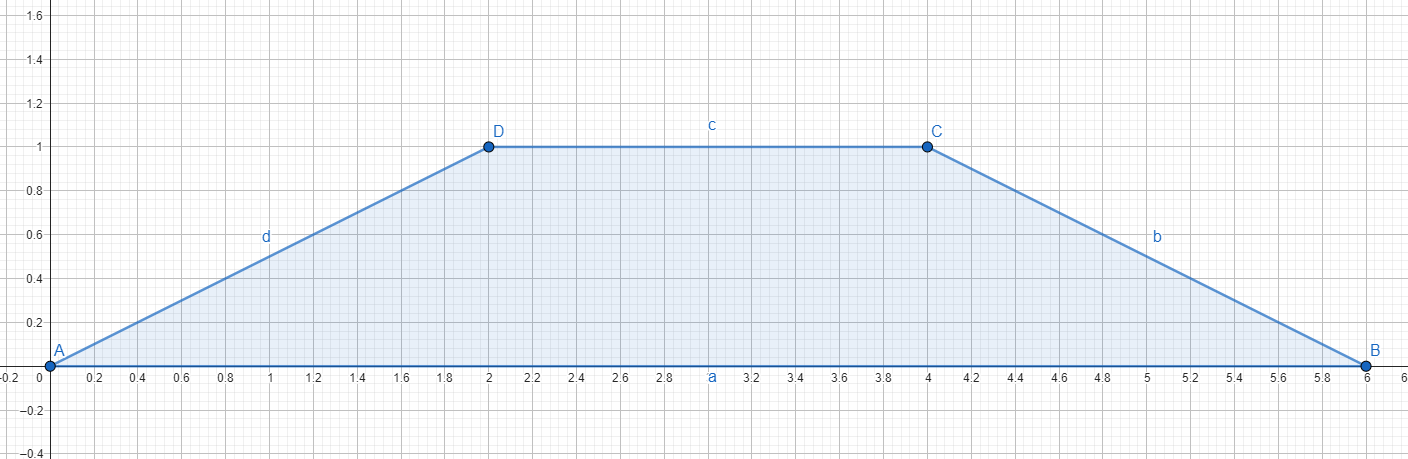
\includegraphics[width=1\linewidth]{img/interpolazione/normalSpeed.png}
    \caption{Sulle Y la nostra velocità, sulle X il tempo. Questo è un normale esempio di un ciclo di accelerazione: acceleriamo fino a che non raggiungiamo maxSpeed ($normalizedSpeed = 1$) e rimaniamo a velocità costante fino a che non deceleriamo del tutto. La distanza percorsa (detta \textit{normalizzata}, poiché la nostra velocità
     massima è pari a 1) corrisponde all'integrale della funzione disegnata dall'andamento della velocità. Per ottenere lo spazio percorso effettivo (detto anche \textit{fisico}), basta moltiplicare la distanza normalizzata per \lstinline{maxPhysicalSpeed}.}
    \label{fig:4_normalSpeed}
\end{figure}

\noindent L'aggiornamento dello stato dell'interpolazione viene effettuato dentro la funzione \lstinline{Update()}, che può essere chiamata ad intervalli di tempo irregolari. Chiameremo \say{tick} oppure \say{frame} il momento in cui viene chiamata \lstinline{Update()}. Il delta tempo tra un frame e l'altro è passato come argomento ad \lstinline{Update()}.

\noindent Prima di iniziare, enuncio dei concetti ricorrenti all'interno di questo capitolo:
\begin{itemize}
    \item L'interpolazione funziona in entrambe le direzioni, ma noi, all'interno della spiegazione, consideriamo solamente il caso in cui andiamo avanti (\say{FORWARD}). Se \lstinline{float currentAcceleration;} è positiva vuol dire che stiamo accelerando, altrimenti stiamo decelerando. Se la nostra direzione fosse opposta, \lstinline{currentAcceleration} e \lstinline{currentSpeed} avrebbero i segni invertiti.
    \item $timeToFullyAccelerate$ (\say{TTFA}): È il tempo richiesto per raggiungere maxSpeed a partire da fermi e viceversa, e si calcola come:
    $TODO$
    Per ottenere quanto tempo ci mettiamo a raggiungere velocità massima o minima a partire da una velocità intermediaria, basta moltiplicare tale velocità per TTFA, poiché tutti i nostri calcoli sono nel range [0, 1].
    \[TimeToAccelerate = \frac{TTFA * (1 - currentSpeed)}{1} = TTFA * (1 - currentSpeed)\]
    \[TimeToStop = \frac{TTFA * currentSpeed}{1} = TTFA * currentSpeed\]
    \begin{figure}[H]
        \centering
        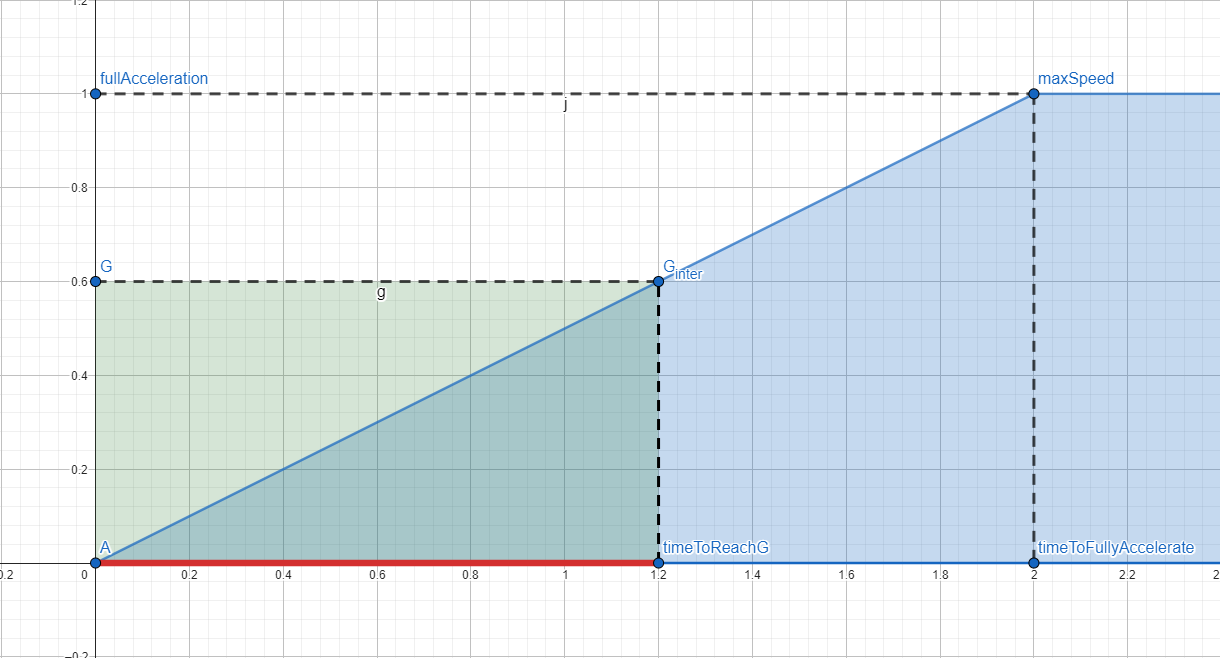
\includegraphics[width=.65\linewidth]{img/interpolazione/timeToFullyAccelerate.png}
        \caption{Grafico che mostra visivamente il calcolo di \textit{TimeToAccelerate}.}
        \label{fig:4_timeToFullyAccelerate}
    \end{figure}
    \item Convertire la velocità interna a velocità reale, ovvero la distanza fisica percorsa al secondo: per le stesse motivazioni di sopra, basta moltiplicare la velocità interna con \lstinline{maxPhysicalSpeed}. Questo ragionamento si applica per tutto, anche per le distanze.
\end{itemize}

Analizziamo la funzione di Update originale (visibile nella figura \ref{fig:4_Update}). Gli step saranno numerati per indicare nei capitoli successivi dove verranno aggiunte le modifiche al codice per compensare il fatto che \lstinline{Update()} venga chiamata ad intervalli irregolari e risolvere altre imprecisioni.
\newcommand{\itemEnu}{\stepcounter{enumi}\textbf{(\number\numexpr\value{enumi}\relax) }}
\begin{enumerate}
    \item Controlliamo se \lstinline{CurrentValue} ha raggiunto \lstinline{TargetValue}. Se sì, ritorniamo, altrimenti \itemEnu controlliamo se l'interpolazione è abilitata. Se no, impostiamo \lstinline{TargetValue = CurrentValue} e ritorniamo.
    \item Calcoliamo quanta distanza abbiamo percorso dall'ultimo tick usando \lstinline{calcNextMovement()}.
    \item Calcoliamo quanta distanza percorreremmo se iniziassimo a decelerare in questo tick, usando \lstinline{getStopDistance()}.
    \item Controlliamo se siamo fermi o meno.
    \item Se siamo fermi, controlliamo se abbiamo raggiunto TargetValue. Se sì, \itemEnu terminiamo l'interpolazione. Altrimenti, \itemEnu calcoliamo la nuova direzione (\lstinline{FORWARD} o \lstinline{BACKWARD}) e \itemEnu forziamo l'inizio dell'interpolazione.
    \item Se non siamo fermi, controlliamo se la distanza calcolata precedentemente è più grande della differenza tra CurrentValue e TargetValue. Se sì, \itemEnu vuol dire che dobbiamo iniziare a decelerare, altrimenti sorpasseremo TargetValue.
    \item Controlliamo il nostro status, ovvero se stiamo accelerando (\lstinline{status == true}) o decelerando (\lstinline{status == false}). Se lo stato è cambiato rispetto allo scorso tick oppure se stiamo forzando l'inizio dell'interpolazione, \itemEnu iniziamo ad accelerare o decelerare impostando, nel primo caso, \lstinline{currentAcceleration = acceleration}, altrimenti, nel secondo caso, \lstinline{currentAcceleration = -acceleration}.
    \item Controlliamo se l'interpolazione è finita testando se stiamo fermi e abbiamo raggiunto TargetValue. Se sì, ritorniamo, altrimenti \itemEnu aggiungiamo a CurrentValue la distanza percorsa nel tick corrente.
\end{enumerate}

Nella funzione \lstinline{Update()} sono state chiamate altre funzioni:
\begin{itemize}
    \item \lstinline{calcNextMovement()}: Questa funzione si occupa di aggiornare la velocità corrente e calcolare la distanza percorsa tra questo frame ed il precedente. La nuova velocità è calcolata come:
    \[speed_{N+1} = speed_{N} + acceleration * DeltaSeconds\]
    Se dopo questo calcolo siamo usciti dal range [0, 1] vuol dire che tra questo tick ed il precedente ci siamo fermati del tutto oppure abbiamo raggiunto la velocità massima. In questo caso effettuiamo un clamp sulla velocità e calcoliamo quanto tempo ci mettiamo a raggiungere il limite del range a partire dalla velocità precedente:
    \[remainingTime = speedToRange * TTFA\]
    Se ci siamo fermati, chiamiamo \lstinline{__calcNextMovement_internal()} con solamente il remainingTime. Se invece abbiamo raggiunto la velocità massima, chiamiamo \lstinline{__calcNextMovement_internal()} per calcolare lo spazio percorso fino a che non abbiamo raggiunto maxSpeed ed aggiorniamo DeltaSeconds come la differenza da quel momento al tick corrente:
    \[DeltaSeconds_{new} = DeltaSeconds_{old} - remainingTime\]
    Infine, se ci stiamo muovendo, chiamiamo \lstinline{__calcNextMovement_internal()} per calcolare ciò che resta del nostro movimento. Quest'ultima chiamata è valida sia quando non raggiungiamo i limiti della velocità e sia quando raggiungiamo maxSpeed.
    \begin{figure}[H]
        \centering
        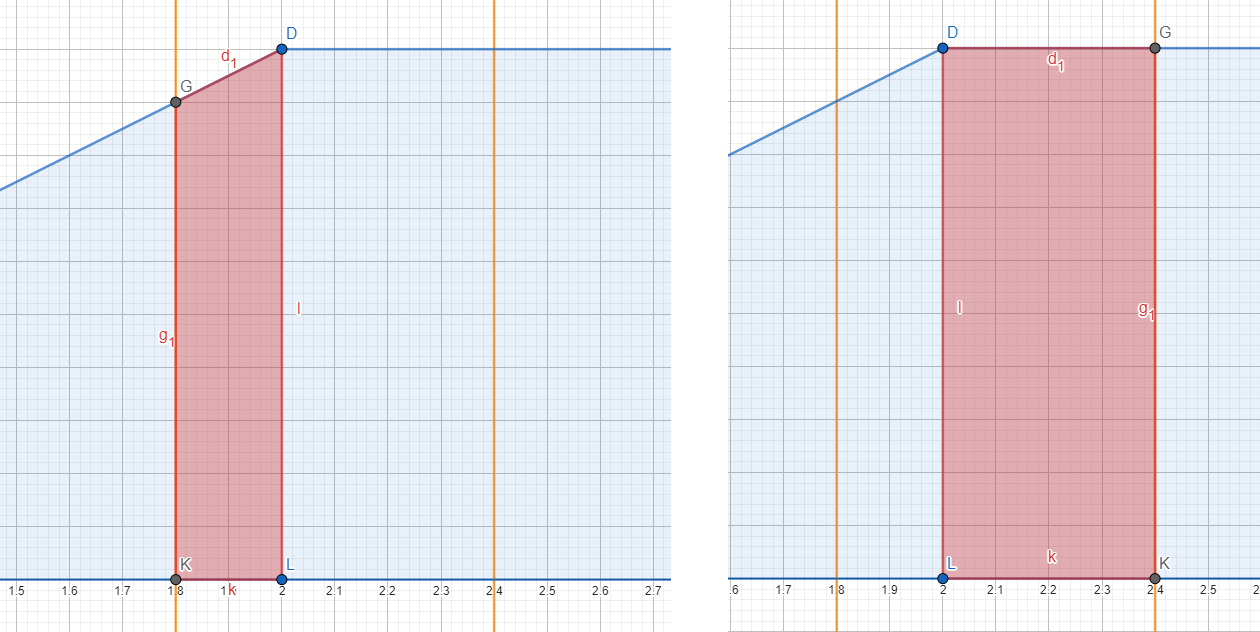
\includegraphics[width=.8\linewidth]{img/interpolazione/calcNextMovementLateCall.png}
        \caption{I due quadrilateri in cui la velocità viene divisa per calcolarne l'area quando raggiungiamo maxSpeed tra un tick e l'altro.}
        \label{fig:4_calcNextMovementLateCall}
    \end{figure}
    \item \lstinline{__calcNextMovement_internal()}: Questa funzione si occupa di calcolare lo spazio percorso in DeltaSeconds a partire dalla velocità precedente fino ad arrivare alla velocità corrente. Il calcolo viene effettuato scomponendo il quadrilatero in un rettangolo con un altezza pari a \lstinline{previousSpeed} a cui va sommata l'area di un triangolo che come altezza ha la differenza tra \lstinline{currentSpeed} e \lstinline{prevSpeed}. Questo calcolo funziona sia quando si accelera, che quando si è a velocità costante (il triangolo avrà area 0 poiché la sua altezza è nulla), che quando si decelera (il calcolo dell'area del triangolo ci darà un valore negativo).
    \[movement = prevSpeed * deltaSeconds + \frac{(currentSpeed - prevSpeed) * deltaSeconds}{2}\]
    \begin{figure}[H]
        \centering
        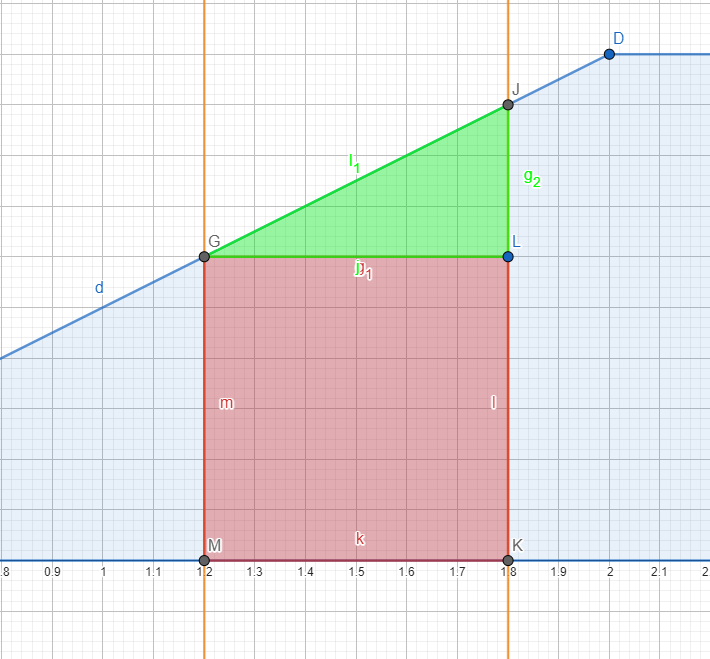
\includegraphics[width=.5\linewidth]{img/interpolazione/calcNextMovementInternalB.png}
        \caption{Scomposizione dell'area per il calcolo del movimento tra un tick e l'altro.}
        \label{fig:4_calcNextMovementInternalB}
    \end{figure}
    \item \lstinline{getStopDistance()}. Questa funzione calcola il movimento percorso se iniziassimo a decelerare dal frame corrente senza poi riaccelerare. Calcola l'area di un triangolo che come altezza ha la velocità corrente e come base ha TTS (TimeToStop).
    \[stopDistance = \frac{TTFA * currentSpeed^2}{2} * maxPhysicalSpeed\]
    \begin{figure}[H]
        \centering
        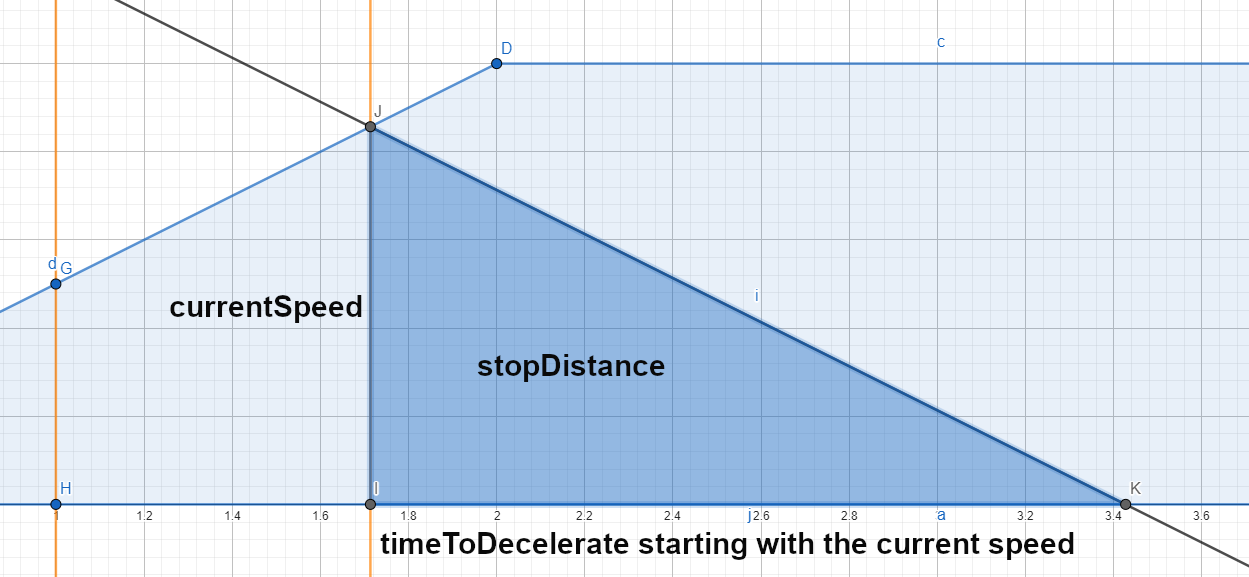
\includegraphics[width=.65\linewidth]{img/interpolazione/getStopTimeLabel.png}
        \caption{Grafico che espone in maniera visiva il calcolo di \textit{stopDistance}.}
        \label{fig:4_getStopTimeLabel}
    \end{figure}
\end{itemize}

\subsection{Modifiche all'implementazione}\label{subsec:4_edits}
Come detto in precedenza, il codice scritto finora proviene da un altro progetto e funziona a patto che i DeltaSeconds tra un tick e l'altro siano costanti e ravvicinati. Questo non è il caso di UnrealEngine e, di conseguenza, bisogna aggiungere delle modifiche all'algoritmo originale per ottenere una interpolazione corretta.

\subsubsection{Compensate Late Call}\label{subsubsec:4_2_CompensateLateCall}
Quasi sempre accade che il momento esatto in cui dovremmo iniziare a decelerare si trovi tra il tick precedente e quello corrente. Iniziando a decelerare in questo tick ci ritroveremo alla fine con più distanza percorsa del dovuto, sorpassando TargetValue.
\begin{figure}[H]
    \centering
    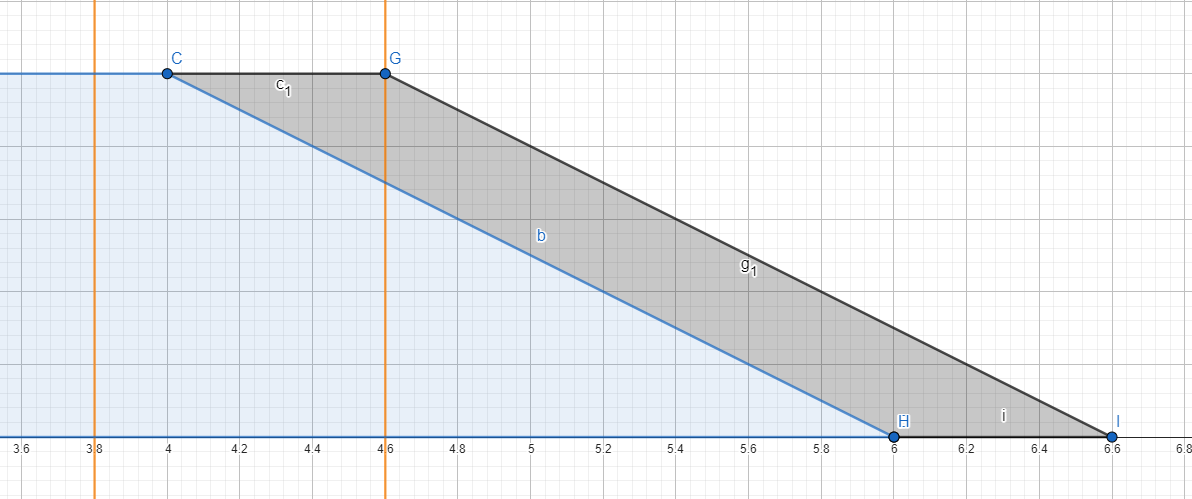
\includegraphics[width=.65\linewidth]{img/interpolazione/compensateLateCall.png}
    \caption{In grigio il movimento extra che viene erroneamente fatto iniziando ad decelerare in ritardo.}
    \label{fig:4_compensateLateCall}
\end{figure}

\noindent Questa correzione viene effettuata quando iniziamo a decelerare e se la stopDistance supera TargetValue (chiameremo la differenza tra i due valori \say{distanceDifference}), ma non abbiamo ancora superato TargetValue. Viene effettuata tra le operazioni in cui viene deciso che dobbiamo iniziare a decelerare e immediatamente prima di cambiare il valore di accelerazione (tra i punti \textbf{12} e \textbf{13} della funzione di \lstinline{Update()}). La prima cosa che fa è effettuare un rollback di qualsiasi movimento svolto durante questo frame e successivamente viene controllato se nel tick precedente stavamo accelerando e se nel tick corrente stiamo a velocità costante. Se sì, vuol dire che tra i due frame abbiamo raggiunto la velocità massima e dobbiamo scoprire se avremmo dovuto iniziare a decelerare prima o dopo averla raggiunta. Per eseguire questo controllo usiamo \lstinline{__calcNextMovement_internal()} per calcolarci lo spazio percorso fino a raggiungere maxSpeed e sommiamo questo valore a quello ottenuto da una chiamata a \lstinline{getStopDistance()} con velocità pari ad 1. Se questa distanza appena calcolata sommata a CurrentValue è più grande di TargetValue vuol dire che avremmo dovuto iniziare a decelerare prima di raggiungere la velocità massima, e viceversa. Nel primo caso ricalcoliamo la distanceDifference come la differenza tra la precedente somma e TargetValue, nel secondo caso faremo semplicemente finta di essere a velocità costante già dal frame precedente.
\begin{figure}[H]
    \centering
    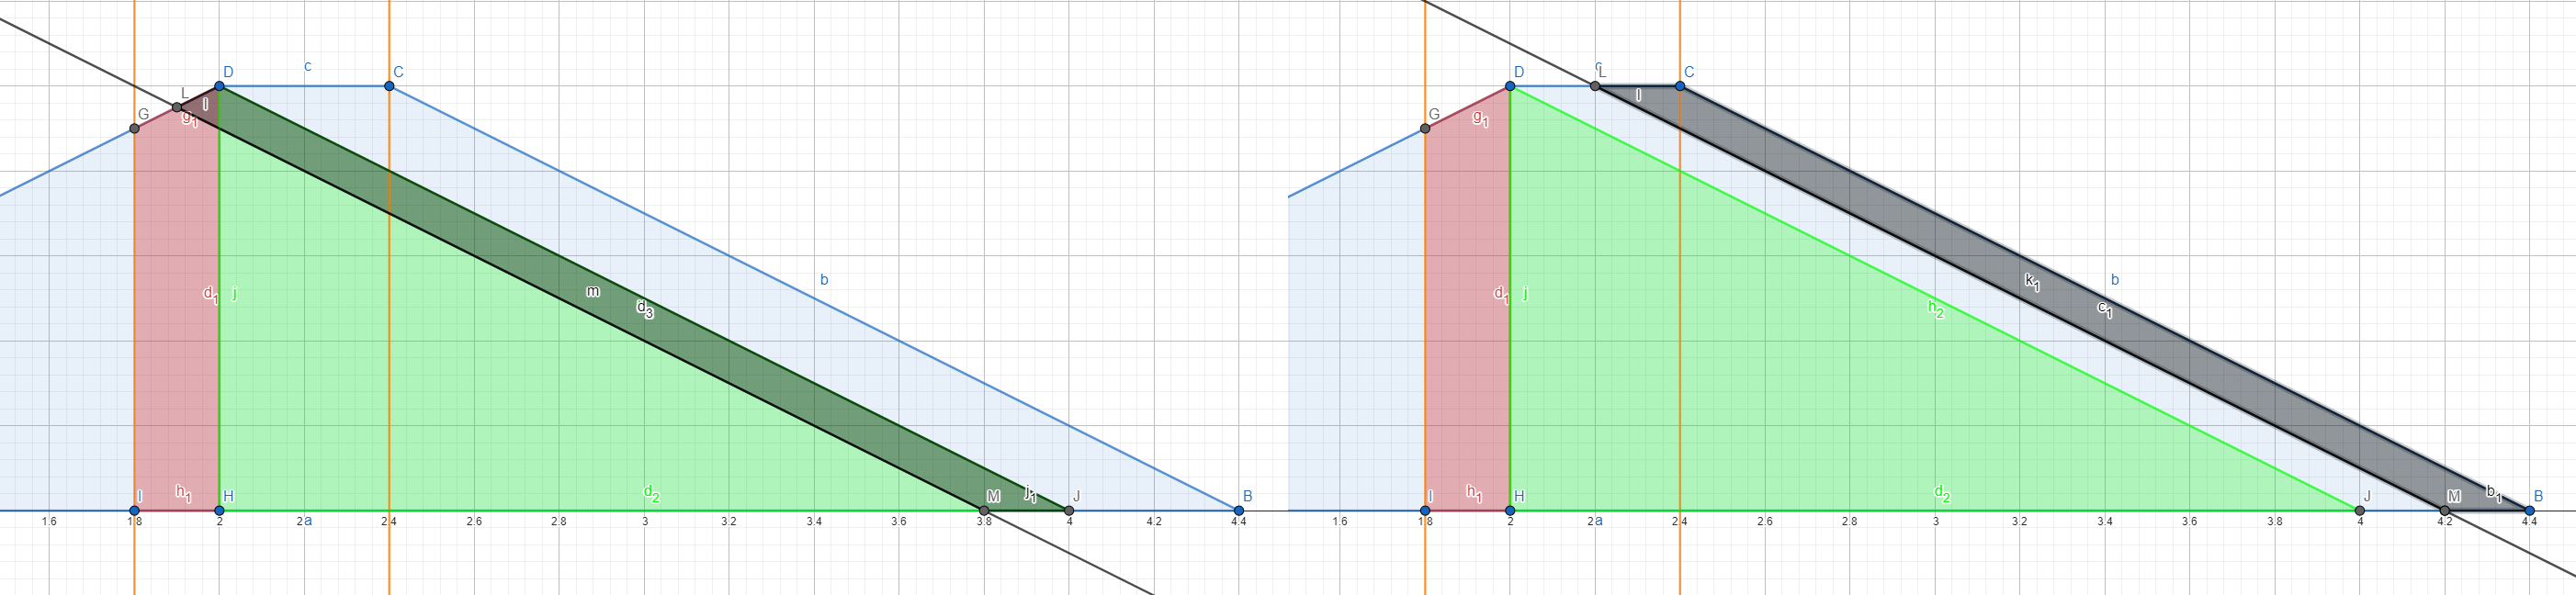
\includegraphics[width=1\linewidth]{img/interpolazione/compensateLateCall3Case.png}
    \caption{In rosso lo spazio percorso fino a raggiungere maxSpeed, in verde la stopDistance a partire da maxSpeed. La somma dei due è quella testata nei precedenti check. In grigio la differenza con TargetValue: a sinistra abbiamo il caso in cui avremmo dovuto iniziare a decelerare prima di raggiungere maxSpeed, a destra dopo.}
    \label{fig:4_compensateLateCall3Case}
\end{figure}

Per calcolare il momento esatto in cui avremmo dovuto iniziare a decelerare avremo due casi possibili: 
%TODO manage to align the following minipages to the right
\begin{itemize}
    \item \textbf{Siamo a velocità costante}: La differenza di spazio percorso è un parallelogramma (vedi la seconda immagine della figura \ref{fig:4_compensateLateCall3Case}) di cui sappiamo l'area (distanceDifference) e l'altezza (1, ovvero maxSpeed). Possiamo calcolarci la base corrispondente alla differenza tra DeltaSeconds ed il momento in cui avremmo dovuto iniziare a decelerare, con una semplice formula inversa:
    \[timeDifference = \frac{distanceDifference}{speed}\]
    
    \begin{minipage}{.45\textwidth}
        \item \textbf{Stiamo accelerando}: Poiché in questo caso stiamo trattando un poligono irregolare (vedi figura \ref{fig:4_compensateLateCallAccel1}), non possiamo applicare direttamente formule inverse. Scomponiamo quindi tale quadrilatero in un triangolo ed un quadrato come nella figura \ref{fig:4_compensateLateCallAccel2} e mettiamo a sistema tutte le dimensioni che sappiamo di tale figura.
    \end{minipage}
    \hfill%
    \begin{minipage}{.475\textwidth}
        \begin{figure}[H]
            \centering
            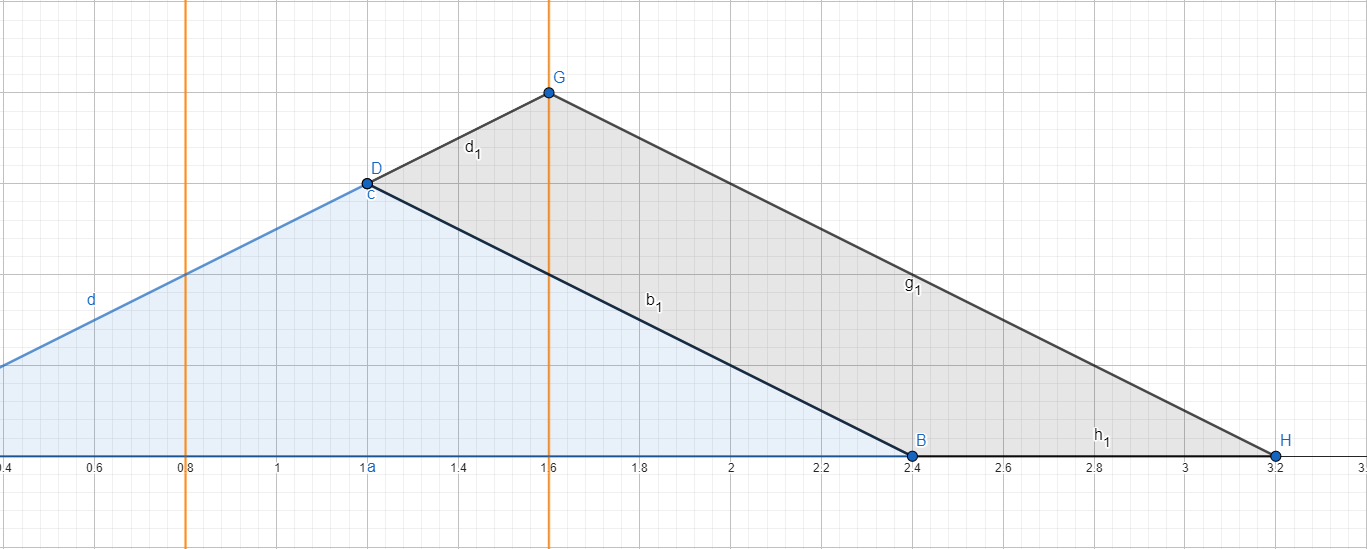
\includegraphics[scale=0.2]{img/interpolazione/compensateLateCallAccel1.png}
            \caption{CompensateLateCall quando stiamo accelerando.}
            \label{fig:4_compensateLateCallAccel1}
        \end{figure}
    \end{minipage}

    \begin{minipage}{.475\textwidth}
        \[B = x\]
        \[H_t = \frac{a}{2}B\]
        \[A_t = \frac{BH_t}{2} = \frac{a}{4}x^2\]
        \[H_r = y\]
        \[A_r = BH_r = xy\]
    \end{minipage}
    \begin{minipage}{.475\textwidth}
        \begin{figure}[H]
            \centering
            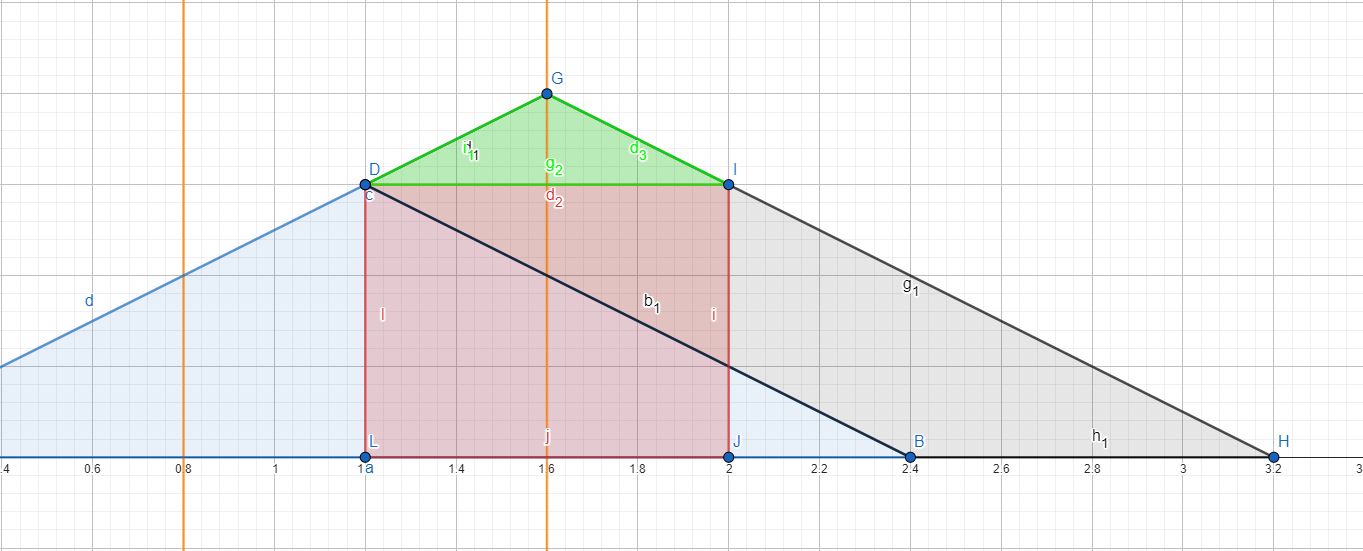
\includegraphics[width=1\linewidth]{img/interpolazione/compensateLateCallAccel2.png}
            \caption{Scomposizione del poligono quando stiamo accelerando.}
            \label{fig:4_compensateLateCallAccel2}
        \end{figure}
    \end{minipage}
    
    Dove $a$ è uguale all'accelerazione; $B$ alla base; $H$, $H_t$ e $H_r$ all'altezza totale, del triangolo e del rettangolo; $A$, $A_t$ e $A_r$ all'area totale, del triangolo e del rettangolo.
    
    Riusciamo a calcolare l'altezza del triangolo a partire dall'accelerazione grazie al fatto che l'accelerazione rappresenta il rapporto tra la crescita della velocità (altezza) rispetto al tempo impiegato (base).\newline
    Le formule per calcolarci l'area totale, corrispondente alla distanceDifference, e l'altezza totale, corrispondente alla velocità al tick corrente, sono:
    \hspace{2cm}
    
    \begin{minipage}{.45\textwidth}\[A = A_t + A_r = \frac{a}{4}x^2 + xy\]\end{minipage}
    \begin{minipage}{.45\textwidth}\[H = H_t + H_r = \frac{a}{4}x^2 + y\]\end{minipage}
    
    Mettendo queste due formule a sistema arriviamo ad ottenere la seguente equazione:
    \[\frac{a}{4}x^2 - Hx + A = 0\]
    Dove $A$, $H$ ed $a$ sono valori noti. Risolvendo l'equazione per x otteniamo quindi la base del nostro poligono, che corrisponde al doppio della differenza in secondi tra il tick corrente e quando avremmo dovuto iniziare a decelerare.
\end{itemize}

\noindent Una volta calcolato quanto tempo prima avremmo dovuto iniziare a decelerare, controlliamo se è un valore positivo. Se sì, ricalcoliamo il movimento fino a quel momento e successivamente iniziamo a decelerare aggiornando il DeltaSeconds della funzione \lstinline{Update()} in modo che calcoli automaticamente il resto dello spostamento. \newline
Se invece il valore risulta negativo, vuol dire che TargetValue è cambiato tra questo ed il frame precedente. Questa casistica viene approfondita e gestita nel capitolo \say{Override Deceleration} \ref{subsubsec:4_2_OverrideDeceleration}.


\subsubsection{Override Deceleration}\label{subsubsec:4_2_OverrideDeceleration}
TargetValue potrebbe cambiare avvicinandosi a CurrentValue sia tra un frame e l'altro che mentre stiamo già decelerando. In entrambi i casi è preferibile decelerare più in fretta piuttosto di fermarsi oltre TargetValue e poi tornare indietro (vedi figura \ref{fig:4_OverrideDecelIntro}).
\begin{figure}[H]
    \centering
    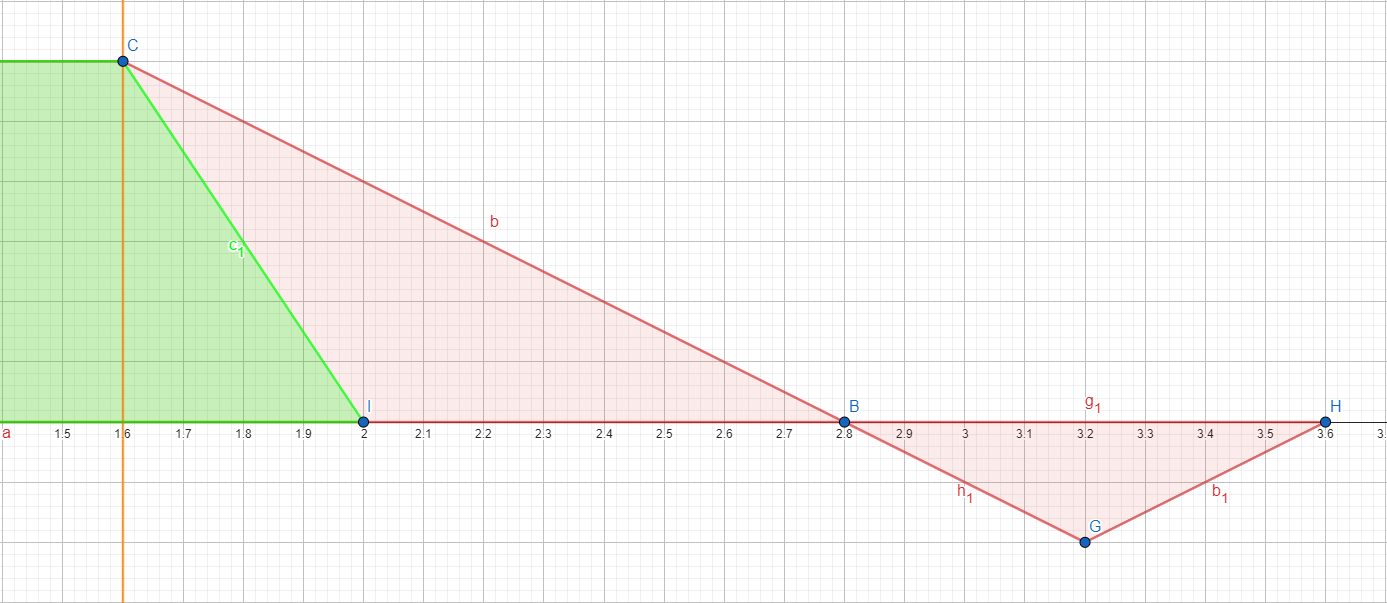
\includegraphics[width=.95\linewidth]{img/interpolazione/OverrideDecelIntro.png}
    \caption{Vogliamo che la nostra velocità si comporti come l'area verde, non come la rossa.}
    \label{fig:4_OverrideDecelIntro}
\end{figure}
%\clearpage %TODO CHECK IF THIS IS STILL NEEDED
\noindent Questa correzione sulla decelerazione viene effettuata quando CompensateLateCall non è stata eseguita oppure ha fallito, stiamo decelerando, TargetValue è cambiato e la nostra stopPosition lo sorpassa. Queste condizioni fanno anche si che mentre stiamo già rallentando la decelerazione possa cambiare di nuovo diventando sia più veloce che più lenta in base ai valori che vengono assegnati a TargetValue. Queste correzioni vengono effettuate come ultimo step nella funzione di \lstinline{Update()}, ergo immediatamente prima del punto \textbf{14}. \newline
La differenza tra questa correzione e CompensateLateCall sta nel fatto che in quest'ultima il momento in cui avremmo dovuto iniziare a decelerare si trova tra il tick corrente ed il precedente, mentre in questo caso si trova prima del frame precedente. Poiché però non possiamo andare \say{indietro nel tempo} e correggere il calcolo effettuato dal tick precedente, l'unica scelta che abbiamo è quella di decelerare più in fretta.\newline

Poiché un motore non può fisicamente decelerare troppo in fretta, è presente un cap hard-coded alla massima velocità di decelerazione pari a $acceleration * 1.5$.

Per calcolarci il nuovo valore di decelerazione, ci serve sapere la stopDistance con una decelerazione normale e la velocità che avevamo nel frame precedente. Calcoliamo quindi la distanceDifference tra la stopDistance e TargetValue e eseguiamo l'operazione inversa per trovarci la base di un triangolo (timeDifference) a partire dalla sua area (distanceDifference) e la sua altezza (prevSpeed). Sottraendo timeDifference a DeltaSeconds ci troviamo il tempo in secondi (punto $G$ nella figura \ref{fig:4_OverrideDecelTimeDiff}) che impiegheremo per raggiungere TargetValue con una velocità che decresce linearmente.
\[stopTime = DeltaSeconds - \frac{distanceDifference * 2}{prevSpeed}\]
\begin{figure}[H]
    \centering
    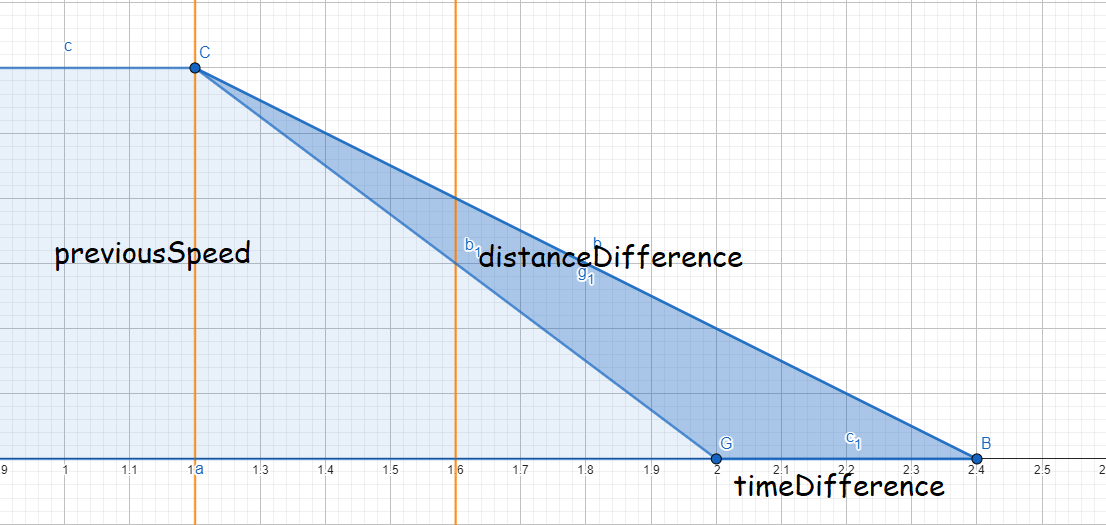
\includegraphics[width=.95\linewidth]{img/interpolazione/OverrideDecelTimeDiff.png}
    \caption{Il punto $G$ è il momento in cui la velocità toccherà lo zero raggiungendo esattamente TargetValue.}
    \label{fig:4_OverrideDecelTimeDiff}
\end{figure}
\clearpage %TODO CHECK IF THIS IS STILL NEEDED
\noindent Il valore di decelerazione corrisponde al coefficiente della retta passante tra il punto in cui iniziamo a decelerare ($C$) e $G$. Assumiamo quindi che $C$ abbia la coordinata X pari a 0. $C$ si troverà quindi a (0, prevSpeed), mentre $G$ si troverà a (stopTime, 0). Possiamo trovare il coefficiente angolare di una retta passante per due punti usando la formula:
\[m = \frac{y_2 - y_1}{x_2 - x_1}\]
Che, nel nostro caso, corrisponde a:
\[acceleration = \frac{0 - prevSpeed}{stopTime - 0} = -\frac{prevSpeed}{stopTime}\]

Una volta trovato questo valore, il codice farà un rollback al tick precedente e ricalcolerà lo spostamento  con il nuovo valore di accelerazione.
%\clearpage %TODO CONTROLLARE SE SERVE ANCORA

\subsubsection{SpeedCap per i piccoli movimenti}\label{subsubsec:4_2_Speedcap}
In una fixture vera, se TargetValue viene spostato di poco, il movimento, al posto di essere a piena velocità, sarà più lento. Questa particolarità è molto utile quando viene effettuato un fade molto lungo che viene gestito da una consolle luci: in questo caso viene inviato costantemente un nuovo valore di TargetValue che si scosta di poco da quello precedente. Con l'attuale implementazione le nostre fixture virtuali si muoverebbero a scatti perché proveranno costantemente a raggiungere TargetValue al meglio della loro velocità, mentre sarebbe più realistico avere un movimento più lento e fluido. 

Per realizzare questa funzionalità si è quindi deciso di imporre uno \say{SpeedCap}, ovvero un limite alla velocità massima di un'interpolazione. Questo limite viene impostato quando il tempo impiegato per raggiungere TargetValue scende sotto una determinata soglia ed è proporzionale alla differenza tra CurrentValue e TargetValue, in modo che il movimento duri almeno quanto tale soglia (vedi figura \ref{fig:4_speedCapIntro}). Il calcolo del valore dello SpeedCap viene effettuato alla fine della funzione \lstinline{SetTargetValue()}, mentre l'attivazione viene svolta nella funzione \lstinline{Update()} dopo aver deciso se dobbiamo iniziare ad accelerare o decelerare, ma prima di effettivamente applicare questa decisione (tra i punti \textbf{11} e \textbf{12}). \newline
\begin{figure}[H]
    \centering
    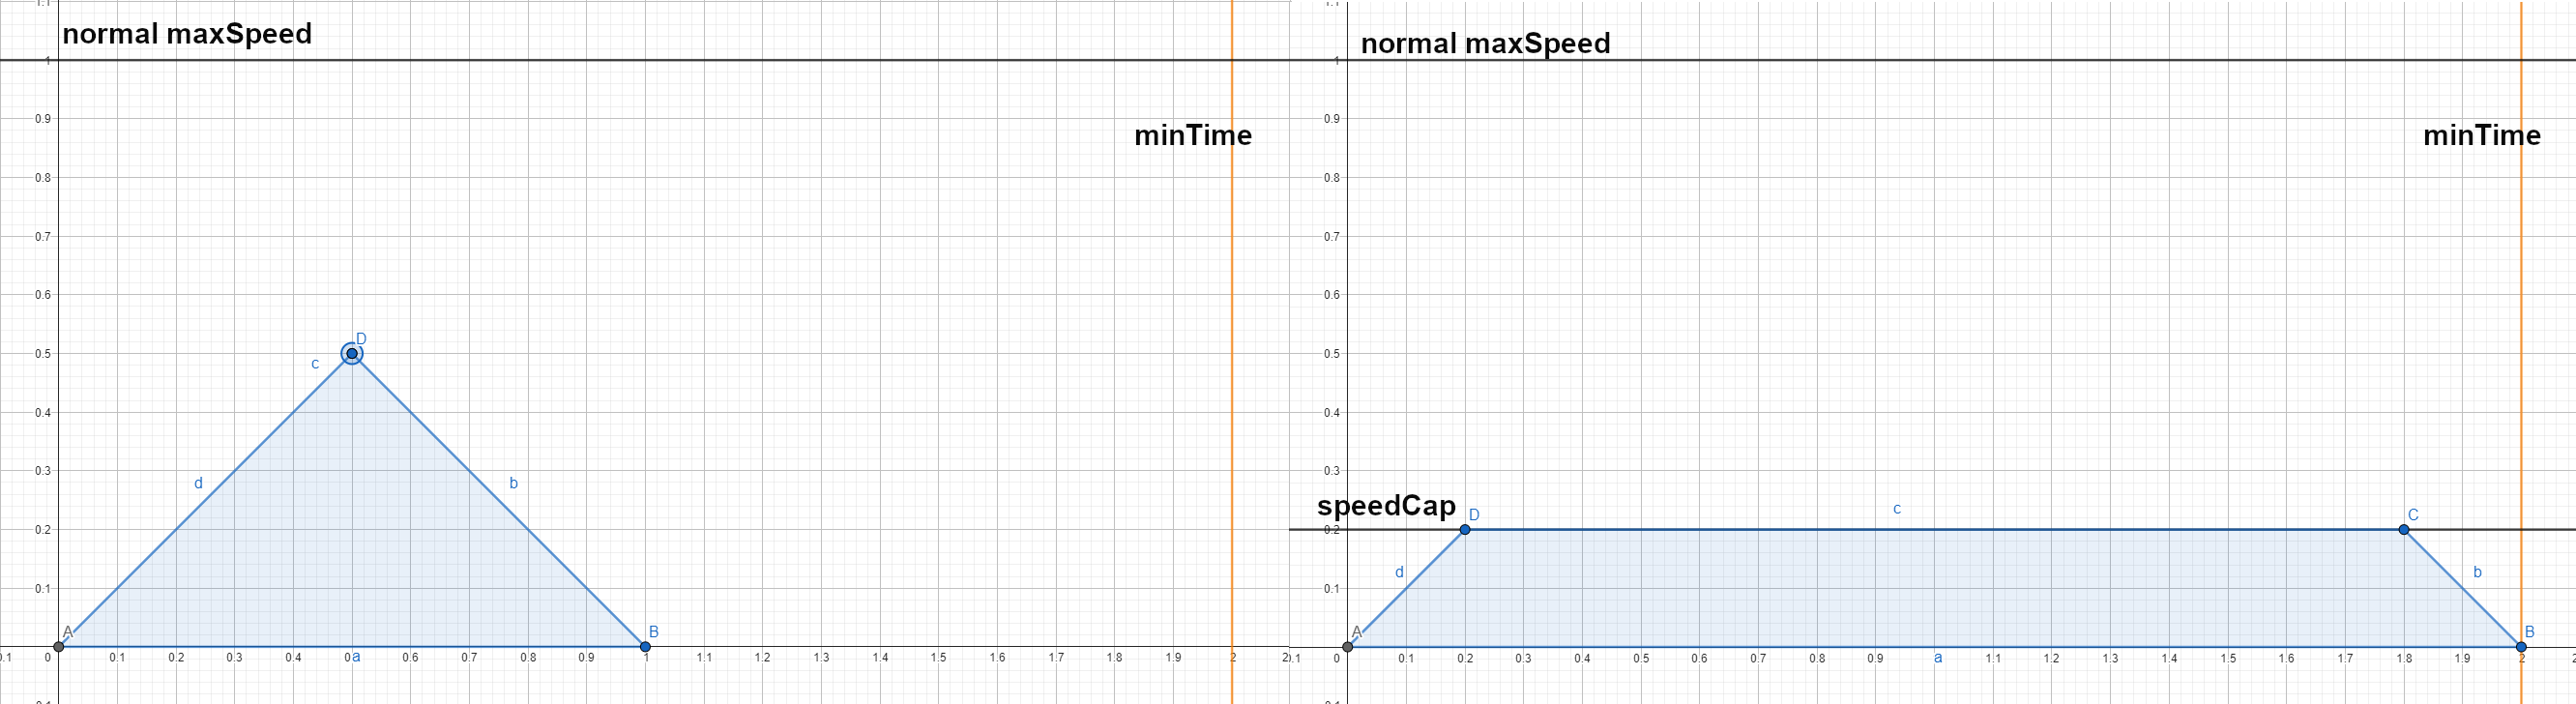
\includegraphics[width=1\linewidth]{img/interpolazione/speedCapIntro.png}
    \caption{A sinistra un ciclo di interpolazione normale, a destra uno con lo speedCap abilitato per effettuare il movimento in \textit{minTime} secondi.}
    \label{fig:4_speedCapIntro}
\end{figure}

\begin{wrapfigure}{r}{0.6\textwidth}
    \centering
    \captionsetup{justification=centering}
    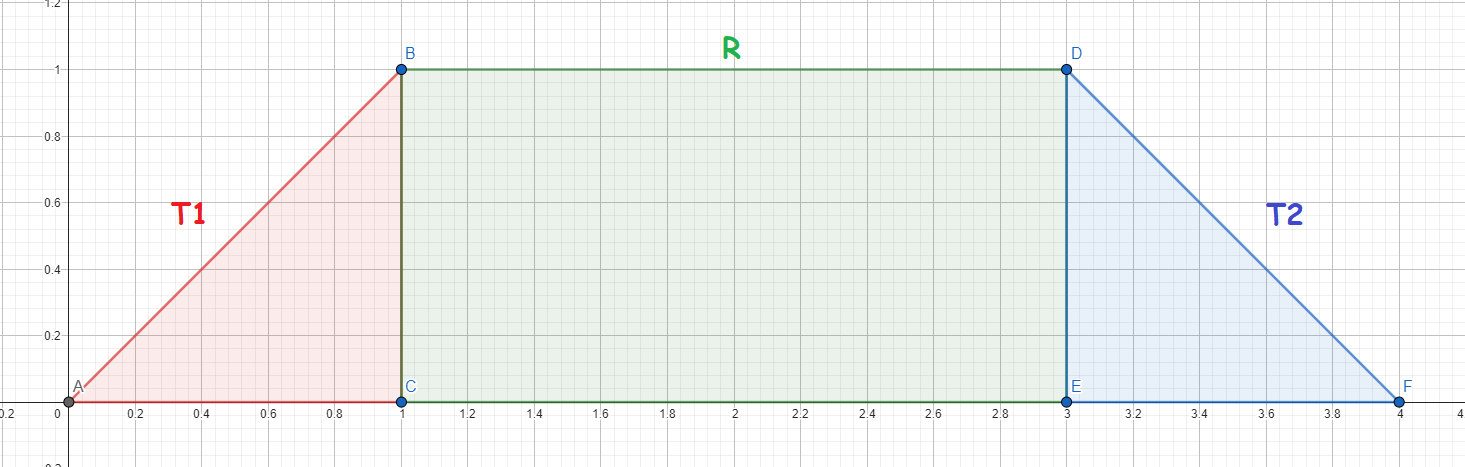
\includegraphics[scale=0.25]{img/interpolazione/movementThreeParts.png}
    \caption{Nel triangolo $T_1$ avviene l'accelerazione, nel rettangolo $R$ rimaniamo a velocità costante e nel triangolo $T_2$ deceleriamo.}
    \label{fig:4_movementThreeParts}
\end{wrapfigure}
\noindent L'ottenimento del tempo impiegato da un intero ciclo di interpolazione viene effettuato attraverso una previsione che prende in considerazione l'accelerazione, la velocità corrente e la differenza tra CurrentValue e TargetValue. Immaginiamo di dividere il ciclo di interpolazione in tre poligoni, come in figura \ref{fig:4_movementThreeParts}. Il raggiungere maxSpeed durante il movimento ci farà calcolare la predizione in maniera differente. \newline

La prima operazione che viene fatta è una compensazione per gestire i casi in cui $currentSpeed > 0$. Calcoliamo quindi due valori: immaginando di partire con velocità pari a 0, otteniamo il tempo per raggiungere currentSpeed (\say{TimeToReachCurrentSpeed}) come:
\[TTRCS = TTFA * currentSpeed\]
E lo spazio percorso fino a raggiungere currentSpeed come l'area di un triangolo che ha TTRCS come base e currentSpeed come altezza:
\[prevArea = \frac{TTRCS * currentSpeed}{2} = \frac{TTFA * currentSpeed^2}{2}\]

\noindent Successivamente avviene il controllo per scoprire se durante l'interpolazione raggiungiamo maxSpeed. La somma dell'area dei due triangoli viene calcolata come:
\[A_t = T_1 + T_2 = 2\frac{TTFA * 1}{2} - prevArea = TTFA - prevArea\]
\begin{figure}[H]
    \centering
    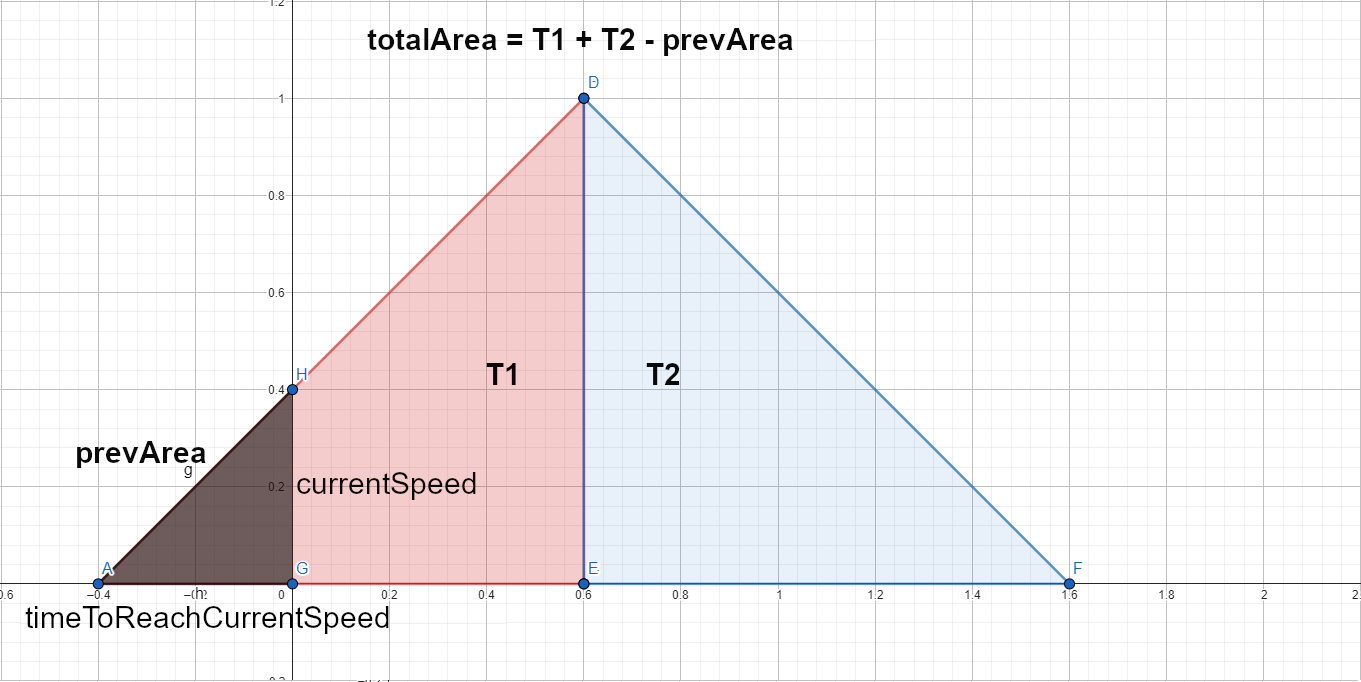
\includegraphics[width=.9\linewidth]{img/interpolazione/speedCapTriangleAreaSplice.png}
    \caption{Calcolo dell'area $T_1 + T_2$ considerando $currentSpeed > 0$.}
    \label{fig:4_speedCapTriangleAreaSplice}
\end{figure}


\textbf{Se l'area di $T_1 + T_2$ è minore di distanceDifference} allora vuol dire che serve arrivare a velocità costante per compiere l'intero movimento. In tal caso abbiamo già la base di $T_1$ e di $T_2$ corrispondenti al tempo di accelerazione e decelerazione; ci manca calcolare la base di $R$: Prima ci calcoliamo l'area di $R$ come $distanceDifference - (T_1 + T_2)$ e successivamente la dividiamo per l'altezza. Poiché stiamo a velocità massima, l'altezza sarà sempre uguale ad 1. La formula finale quindi per calcolare il tempo richiesto da una interpolazione per completare il suo ciclo raggiungendo la velocità massima è quindi:
\[time = (TTFA * 2 - TTRCS) + (distanceDifference - A_t)\]
\begin{figure}[H]
    \centering
    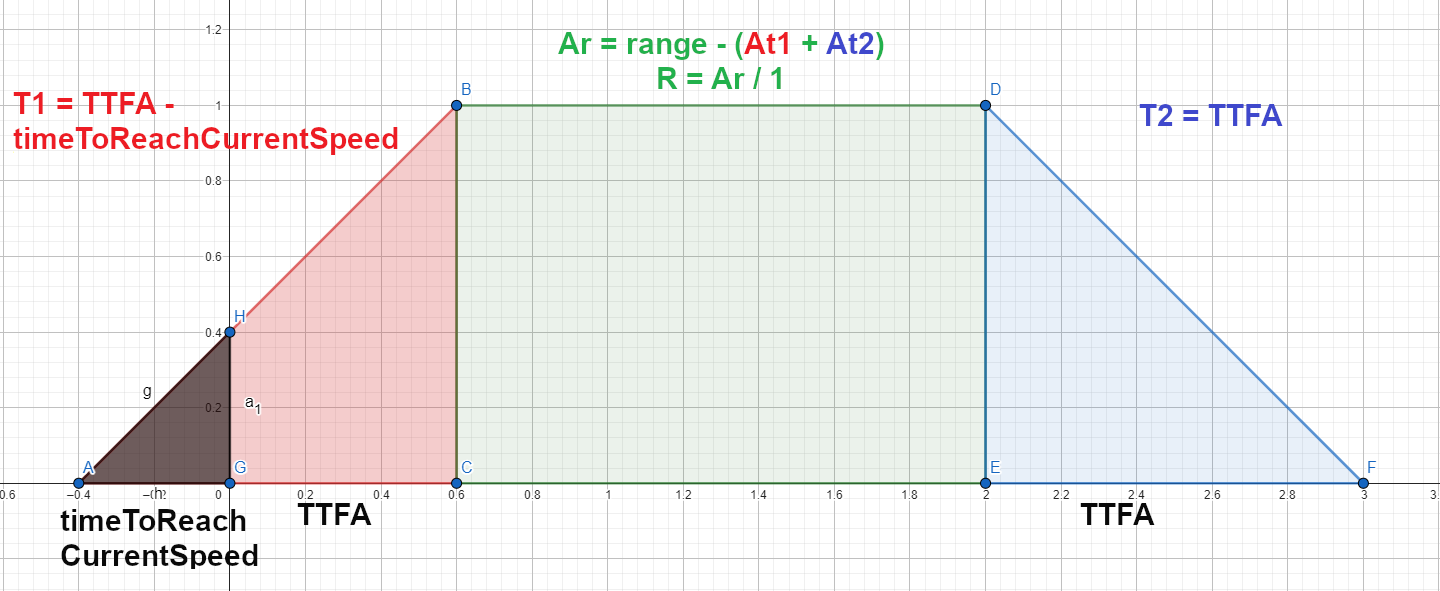
\includegraphics[width=1\linewidth]{img/interpolazione/speedCapTotalAreaCalc.png}
    \caption{Calcolo del tempo richiesto da una interpolazione quando raggiungiamo maxSpeed.}
    \label{fig:4_speedCapTotalAreaCalc}
\end{figure}

\textbf{Se l'area di $T_1 + T_2$ è maggiore o uguale di distanceDifference} allora vuol dire che \textbf{non} serve arrivare a velocità costante per compiere l'intero movimento. Dobbiamo quindi trovare la base (corrispondente al tempo dell'interpolazione) di un triangolo di cui sappiamo l'area ($A$, corrispondente alla distanceDifference) e il rapporto ($a$, corrispondente all'accelerazione) tra la base ($B$, notiamo come l'accelerazione si riferisce alla base di solo uno dei due triangoli) e l'altezza ($H$).
\[H = aB\]
\[A = \frac{2BH}{2}\]
Risolvendo per $B$ arriviamo quindi a:
\[B = \sqrt{\frac{A}{a}}\]
\clearpage
Come detto sopra, $B$ fa riferimento solamente alla base di uno dei due triangoli. Per ottenere quindi il tempo totale bisogna moltiplicare $B$ per 2. Inoltre, se $currentSpeed > 0$ allora bisogna aggiungere il \say{pezzo} di $T_1$ che viene tagliato fuori all'area totale, e togliere da $2B$ il TTRCS. La formula finale è quindi la seguente:
\[B = 2\sqrt{\frac{A + prevArea}{a}} - TTRCS\]
\begin{figure}[H]
    \centering
    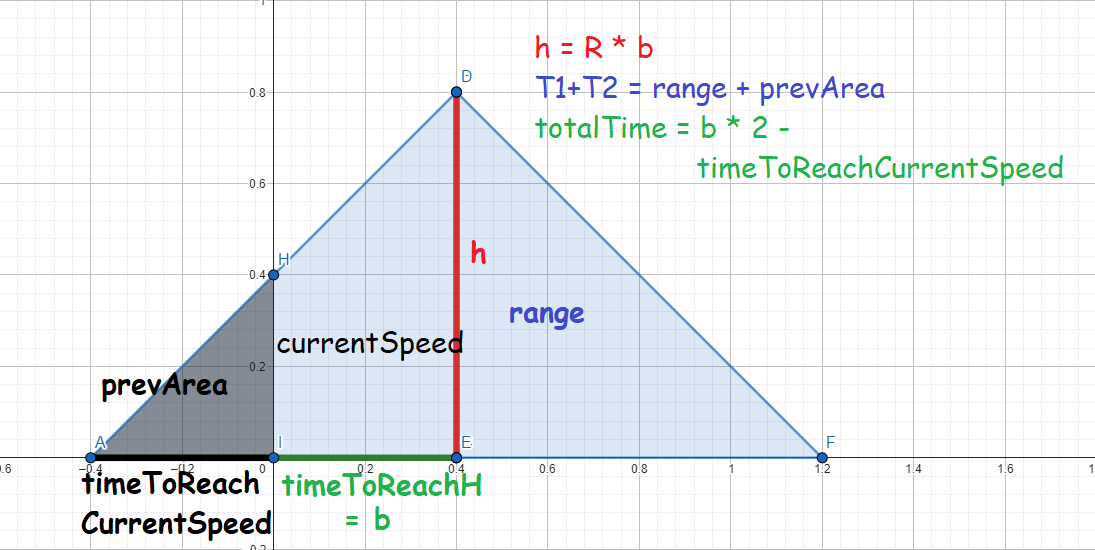
\includegraphics[width=1\linewidth]{img/interpolazione/speedCapNoMaxSpeedCalcSplice.png}
    \caption{Calcolo del tempo richiesto da una interpolazione quando \textbf{non} raggiungiamo maxSpeed.}
    \label{fig:4_speedCapNoMaxSpeedCalcSplice}
\end{figure}

\noindent Come detto sopra, vogliamo che il tempo impiegato da una interpolazione a completare il suo ciclo sia pari almeno a quello di una soglia prestabilita. Se dal nostro calcolo il tempo risultasse inferiore, dobbiamo trovare una velocità massima ($x$) in modo da percorrere il movimento esattamente in quel limite di tempo. Andiamo ad impostare un'equazione con le seguenti variabili:
\begin{itemize}
    \item $x$: Valore finale dello speedCap.
    \item $t$: Alias di TTFA (\textbf{Valore noto}).
    \item $s$: Alias di currentSpeed (\textbf{Valore noto}).
    \item $T$: Tempo totale, ovvero in quanto tempo l'interpolazione deve essere completata (\textbf{Valore noto}).
    \item $B_1$: Base di $T_1$, ottenuta dalla differenza tra TTRCS e TimeToReachX, ovvero il tempo per raggiungere lo speedCap (abbreviato con \say{TTRX}). Poiché la velocità iniziale può essere superiore allo speedCap, questa differenza deve essere assoluta: \[B_1 = t\abs{x - s} = \abs{tx - ts}\]
    \item $B_2$: Base di $T_2$ definita semplicemente come TTRX: \[B_2 = tx\]
    \item $B_r$: Base di $R$ definita come la base totale meno quella dei due triangoli: \[B_r = T - B_1 - B_2 = T - B_1 - tx\]
    \item $A_1$: Area di $T_1$ ottenuta in maniera simile a \lstinline{__calcNextMovementInternal()}, ovvero la somma tra l'area di un rettangolo con l'altezza uguale a currentSpeed e quella di un triangolo con la stessa base e l'altezza uguale alla differenza tra $x$ e la currentSpeed: \[A_1 = sB_1 + \frac{(x - s)B_1}{2}\]
    \item $A_2$: L'area di $T_2$ ottenuta come l'area di un normale triangolo con altezza uguale a $x$: \[A_2 = \frac{B_2x}{2} = \frac{tx^2}{2}\]
    \item $A_r$: L'area di $R$ definita come l'area di un normale rettangolo con altezza uguale a $x$: \[A_r = B_rx = Tx - B_1x - tx^2\]
    \item $A$: Area totale, ovvero lo spazio che l'interpolazione deve percorrere per arrivare a TargetValue (alias di distanceDifference. \textbf{Valore noto}). Definita come la somma delle tre precedenti aree (la formula è già stata semplificata): \[A = A_1 + A_2 + A_r = \frac{sB_1}{2} + \frac{xB_1}{2} + \frac{tx^2}{2} + Tx\]
\end{itemize}
Otteniamo quindi l'equazione:
\[\frac{s\abs{tx - ts}}{2} + \frac{x\abs{tx - ts}}{2} + \frac{tx^2}{2} + Tx - A = 0\]
Possiamo avere 3 possibili casi:\newline
\begin{itemize}
    \item $s > x$: Partendo dalla currentSpeed dobbiamo decelerare fino ad arrivare allo speedCap. Dobbiamo sostituire il modulo nella precedente equazione con $tx - ts$.
    \begin{figure}[H]
        \centering
        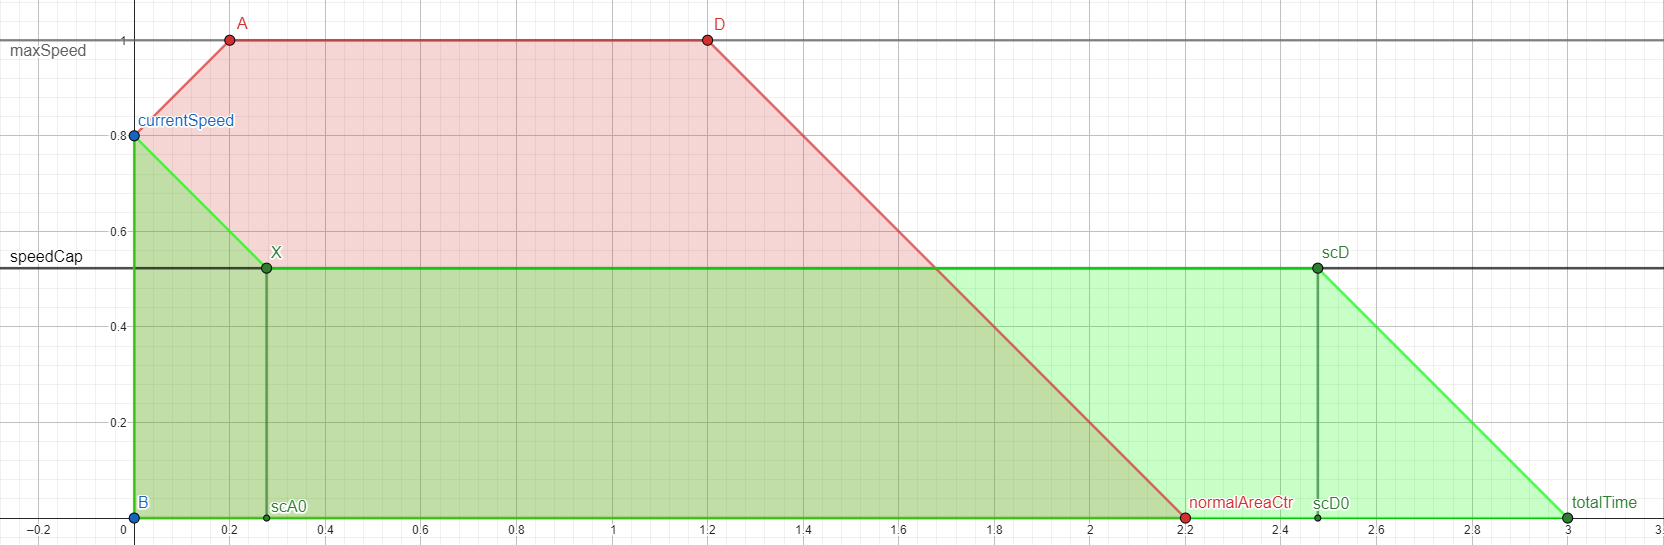
\includegraphics[width=.8\linewidth]{img/interpolazione/speedCapCalcGE.png}
        \caption{In rosso l'andamento velocità senza imporre uno speedCap, che ci fa raggiungere TargetValue troppo velocemente. In verde la velocità con uno speedCap  minore alla velocità corrente che ci farà raggiungere TargetValue nel tempo corretto. Le due aree si equivalgono.}
        \label{fig:4_speedCapCalcGE}
    \end{figure}
%\clearpage %TODO CHECK IF THIS IS REALLY NEEDED
    \item $s < x$: Partendo dalla currentSpeed dobbiamo accelerare fino ad arrivare allo speedCap. Dobbiamo sostituire il modulo nella precedente equazione con $ts - tx$.
    \begin{figure}[H]
        \centering
        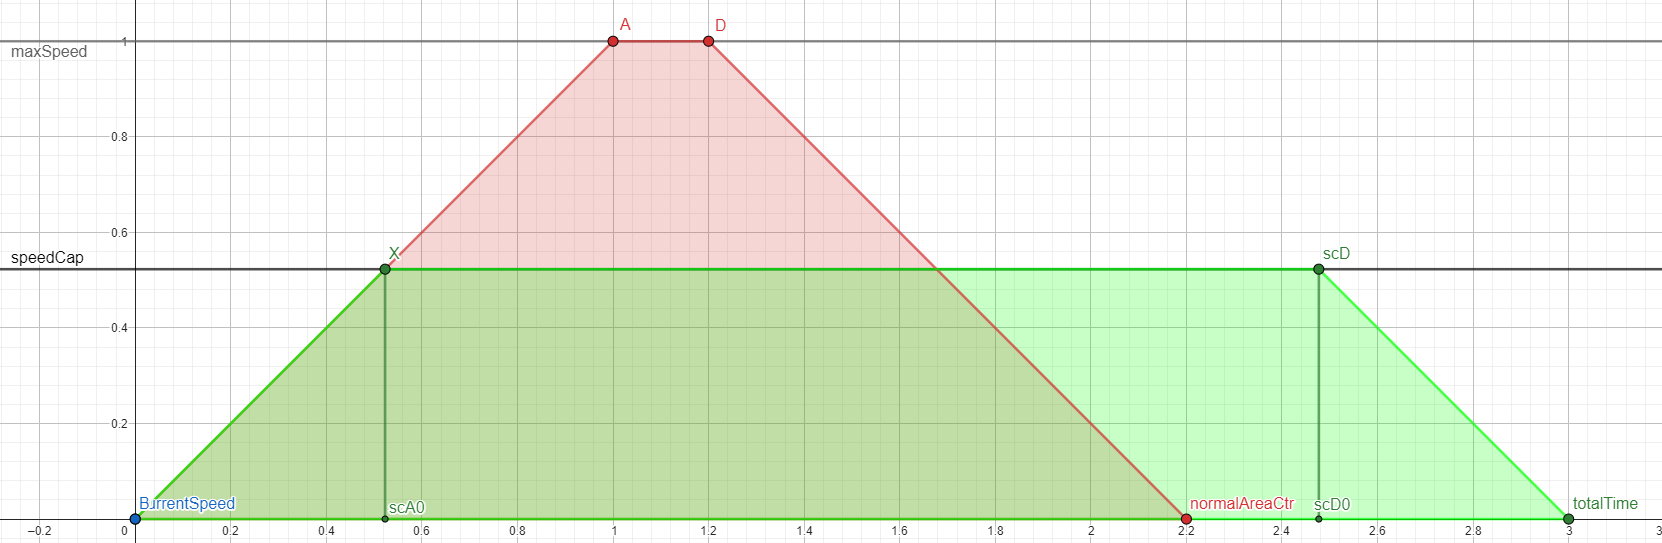
\includegraphics[width=.8\linewidth]{img/interpolazione/speedCapCalcBE.png}
        \caption{Stessa illustrazione della figura \ref{fig:4_speedCapCalcGE}. L'unica differenza è che lo speedCap è maggiore della velocità corrente e di conseguenza lo raggiungeremo accelerando al posto di decelerare.}
        \label{fig:4_speedCapCalcBE}
    \end{figure}

\item $s = x$: currentSpeed è già allo stesso valore di speedCap. Possiamo precedere come uno dei due precedenti casi. \newline
\end{itemize}

\noindent Le equazioni finali per ottenere lo speedCap a partire dalla nostra velocità, l'accelerazione e il tempo in cui dobbiamo percorrere l'interpolazione, sono:
\[tx^2 + (ts + T)x + (\frac{ts^2}{2} + A) = 0 \quad\text{quando}\qquad x \geq p\]
\[(-ts + T)x + (\frac{ts^2}{2} - A) = 0 \quad\text{quando}\qquad x \leq p\]

\noindent Il codice inizialmente risolverà prima il secondo caso poiché più rapido, visto che non implica risolvere un'equazione di secondo grado, e controllerà la validità del risultato. Se il risultato non rispetta la condizione specificata, allora procederà con la risoluzione del primo caso. \newline

Una volta mostrato come lo speedCap viene calcolato ed impostato, la funzione \lstinline{Update()} si dovrà occupare di mantenerlo ed interverrà solamente se non stiamo già decelerando per raggiungere TargetValue. Lo speedCap è implementato impostando l'override dell'accelerazione (lo stesso usato da OverrideDeceleration \ref{subsubsec:4_2_OverrideDeceleration}) a 0. Il codice si occuperà di rimuovere l'override quando lo speedCap viene disattivato dentro \lstinline{TargetValue} e si occuperà di impostarlo o forzare la decelerazione quando viene invece attivato.

\noindent Più specificatamente, abbiamo 3 casi da gestire (visualizzati anche nella figura \ref{fig:4_speedCapThreeCases}):
\begin{enumerate}
    \item \textbf{La nostra velocità ha raggiunto lo speedCap}: Sovrascriviamo l'accelerazione con 0 in modo che la velocità non venga più aggiornata.
    \item \textbf{La nostra velocità è superiore allo speedCap}: Forziamo una decelerazione fino a che non raggiungiamo lo speedCap, ricadendo nel caso \textbf{1}. Questo caso copre anche la situazione in cui eravamo già fermi su uno speedCap e nel mentre \textbf{cambia verso un valore più piccolo}.
    \item \textbf{Avevamo già raggiunto uno speedCap e nel mentre cambia verso un valore più grande}: Disabilitiamo l'override dell'accelerazione in modo da tornare a guadagnare velocità, fino a che non ricadiamo nel caso \textbf{1}.
\end{enumerate}

\noindent Ci sono due casi che sono trattati implicitamente dal resto della funzione \lstinline{Update()} e quindi non serve prendere particolari misure:
\begin{itemize}
    \item Il caso in cui la nostra velocità è inferiore ad uno speedCap e non ne abbiamo ancora mai raggiunto uno, non è coperto perché stiamo normalmente già accelerando. Eventualmente ricadremo nel caso \textbf{1}.
    \item Il caso in cui dobbiamo iniziare a decelerare perché stiamo raggiungendo TargetValue non è coperto perché iniziando a decelerare viene impostata una nuova accelerazione, operazione che disattiva automaticamente l'override della stessa.
\end{itemize}

\begin{figure}[H]
    \centering
    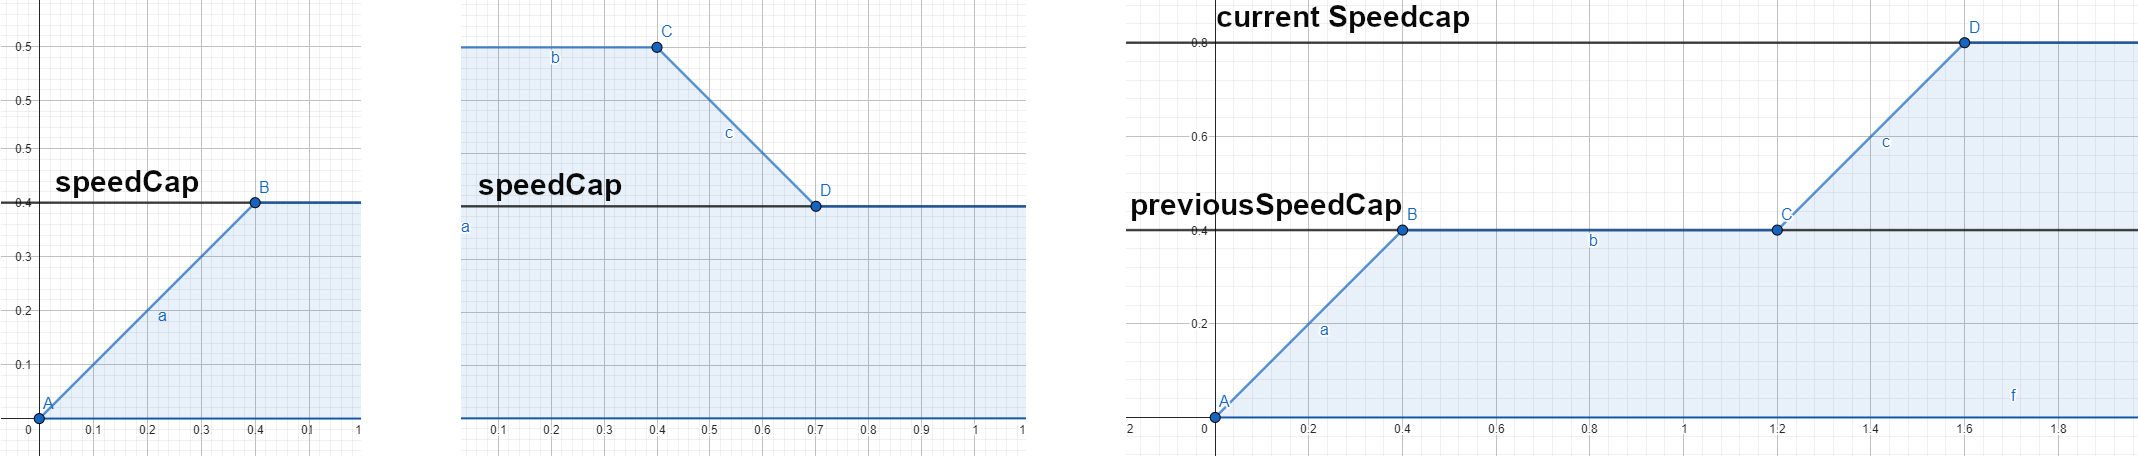
\includegraphics[width=1\linewidth]{img/interpolazione/speedCapThreeCases-split.png}
    \caption{I tre casi descritti sopra, da sinistra verso destra.}
    \label{fig:4_speedCapThreeCases}
\end{figure}

%\clearpage %TODO CHECK IF STILL NEEDED
\subsubsection{Conversioni da RealFade e RealAcceleration}\label{subsubsec:4_2_Conversions}
Questa funzione si occupa di convertire i parametri GDTF \lstinline{RealFade} e \lstinline{RealAcceleration} verso i valori \lstinline{maxSpeed} e \lstinline{acceleration} utilizzati all'interno dell'oggetto interpolazione. Per calcolare \lstinline{maxPhysicalSpeed} c'è bisogno della dimensione del range in cui opererà l'interpolazione, definito come $MaxValue - MinValue$.\newline

\begin{wrapfigure}{r}{0.55\textwidth}
    \centering
    \captionsetup{justification=centering}
    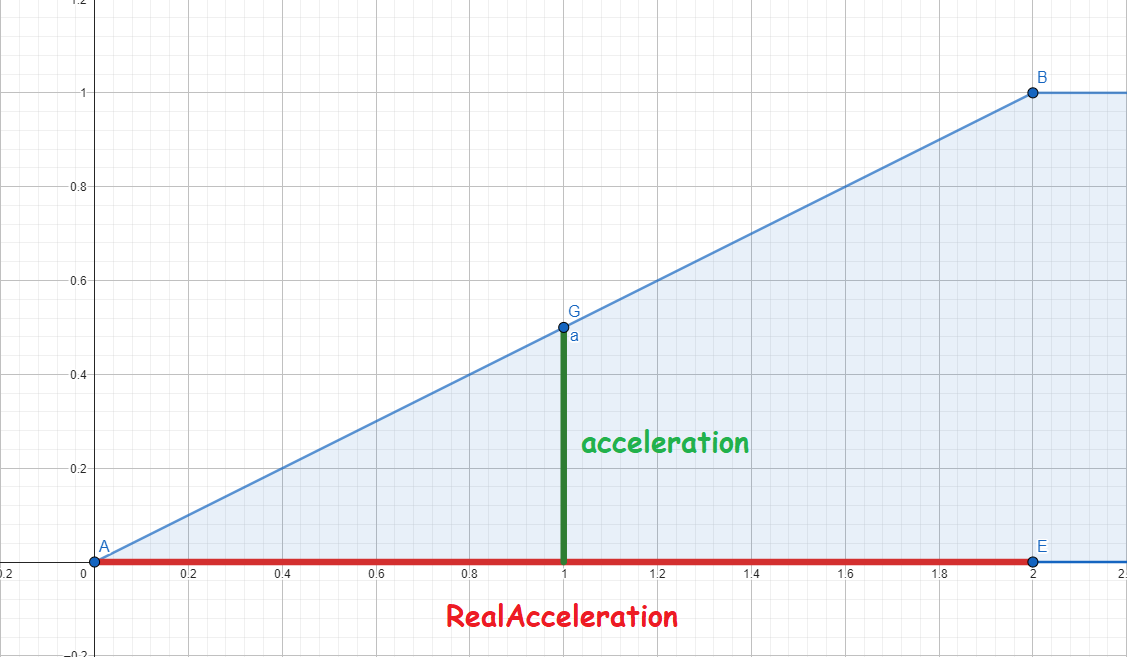
\includegraphics[scale=0.3]{img/interpolazione/RealAccelerationVSacceleration.png}
    \caption{Differenza tra \textit{acceleration} e \textit{RealAcceleration}.}
    \label{fig:4_RealAccelerationVSacceleration}
\end{wrapfigure}
Il parametro \lstinline{RealAcceleration} rappresenta il tempo in secondi utilizzati per passare da 0 a maxSpeed, mentre \lstinline{acceleration} rappresenta quanta velocità guadagniamo ogni secondo. Poiché \lstinline{acceleration} è il reciproco di \lstinline{RealAcceleration}, possiamo ottenerlo semplicemente facendo:
\[acceleration = \frac{1}{RealAcceleration}\] \newline
%\clearpage %TODO CHECK IF STILL NEEDED

Il parametro \lstinline{RealFade} considera anche i tempi di accelerazione e decelerazione di un movimento, per cui non possiamo usarlo direttamente come valore di \lstinline{maxPhysicalSpeed} che, ricordiamo, rappresenta quanto movimento facciamo ogni secondo quando siamo a maxSpeed. Per ottenere questo valore dobbiamo quindi fare una proporzione (RealAcceleration è abbreviato in $a$ e RealFade è abbreviato in $f$):
\begin{itemize}
    \item L'area dei triangoli dell'accelerazione/decelerazione è uguale a $\frac{a * maxSpeed}{2}$. Poiché maxSpeed è uguale ad 1 e ci serve calcolare l'area di entrambi perché entrambi presenti dentro RealFade, la formula sarà:
    \[A_1 + A_2 = 2\frac{a * 1}{2} = a\]
    \item La base di $R$ è uguale a RealFade meno la base di $T_1$ e $T_2$, ergo $f - 2a$. L'area di $R$ invece corrisponde alla base per maxSpeed, che essendo uguale ad 1 ritorniamo con la stessa formula di prima:
    \[B_r = f - B_1 - B_2 = f - 2a\]
    \[A_r = B_r * maxSpeed = B_r * 1 = B_r\]
    \item L'area totale è uguale a:
    \[A = A_1 + A_2 + A_r = a + f - 2a = f - a\]
\end{itemize}
A questo punto mettiamo in proporzione l'area \say{virtuale} appena calcolata con la sua velocità massima (ovvero 1), e il range reale dell'interpolazione con \lstinline{maxPhysicalSpeed}, che vogliamo calcolare:
\[A : maxSpeed = range : maxPhysicalSpeed\]
E risolviamo la proporzione attraverso la formula:
\[maxPhysicalSpeed = \frac{range * maxSpeed}{A} = \frac{range * 1}{A} = \frac{range}{f - a}\]
\begin{figure}[H]
    \centering
    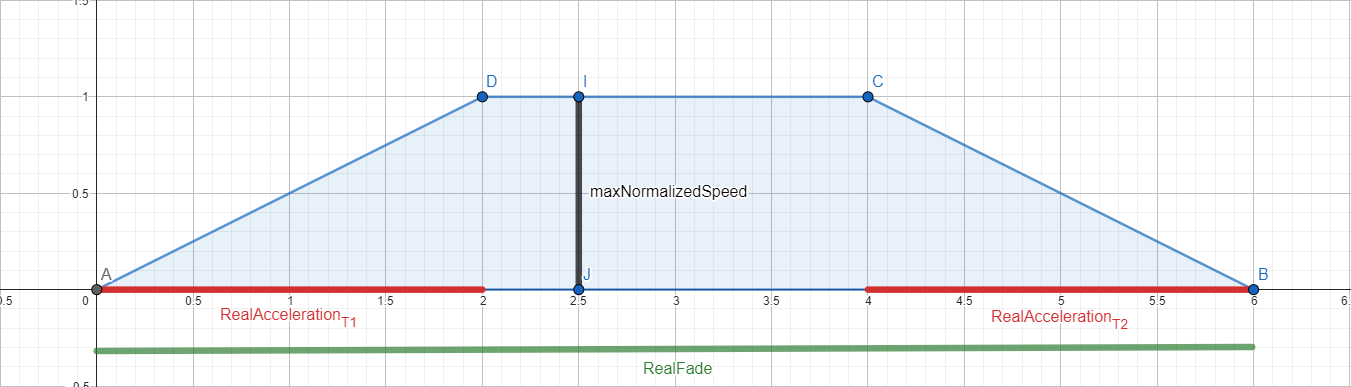
\includegraphics[width=1\linewidth]{img/interpolazione/RealAccelerationVSRealFadeVSmaxSpeed.png}
    \caption{I vari valori della precedente proporzione.}
    \label{fig:4_RealAccelerationVSRealFadeVSmaxSpeed}
\end{figure}
\clearpage %TODO CHECK IF STILL NEEDED

\subsubsection{Codice}\label{subsubsec:4_2_Code}
Qui sotto mostrata la funzione \lstinline{Update()} e \lstinline{SetTargetValue()} in cui è possibile osservare i vari punti esposti nel capitolo \ref{subsec:4_trafficImplementation} ed in cui sono evidenziate le modifiche fatte all'algoritmo originale per implementare le varie funzionalità e correzioni.
\begin{figure}[H]
    \centering
    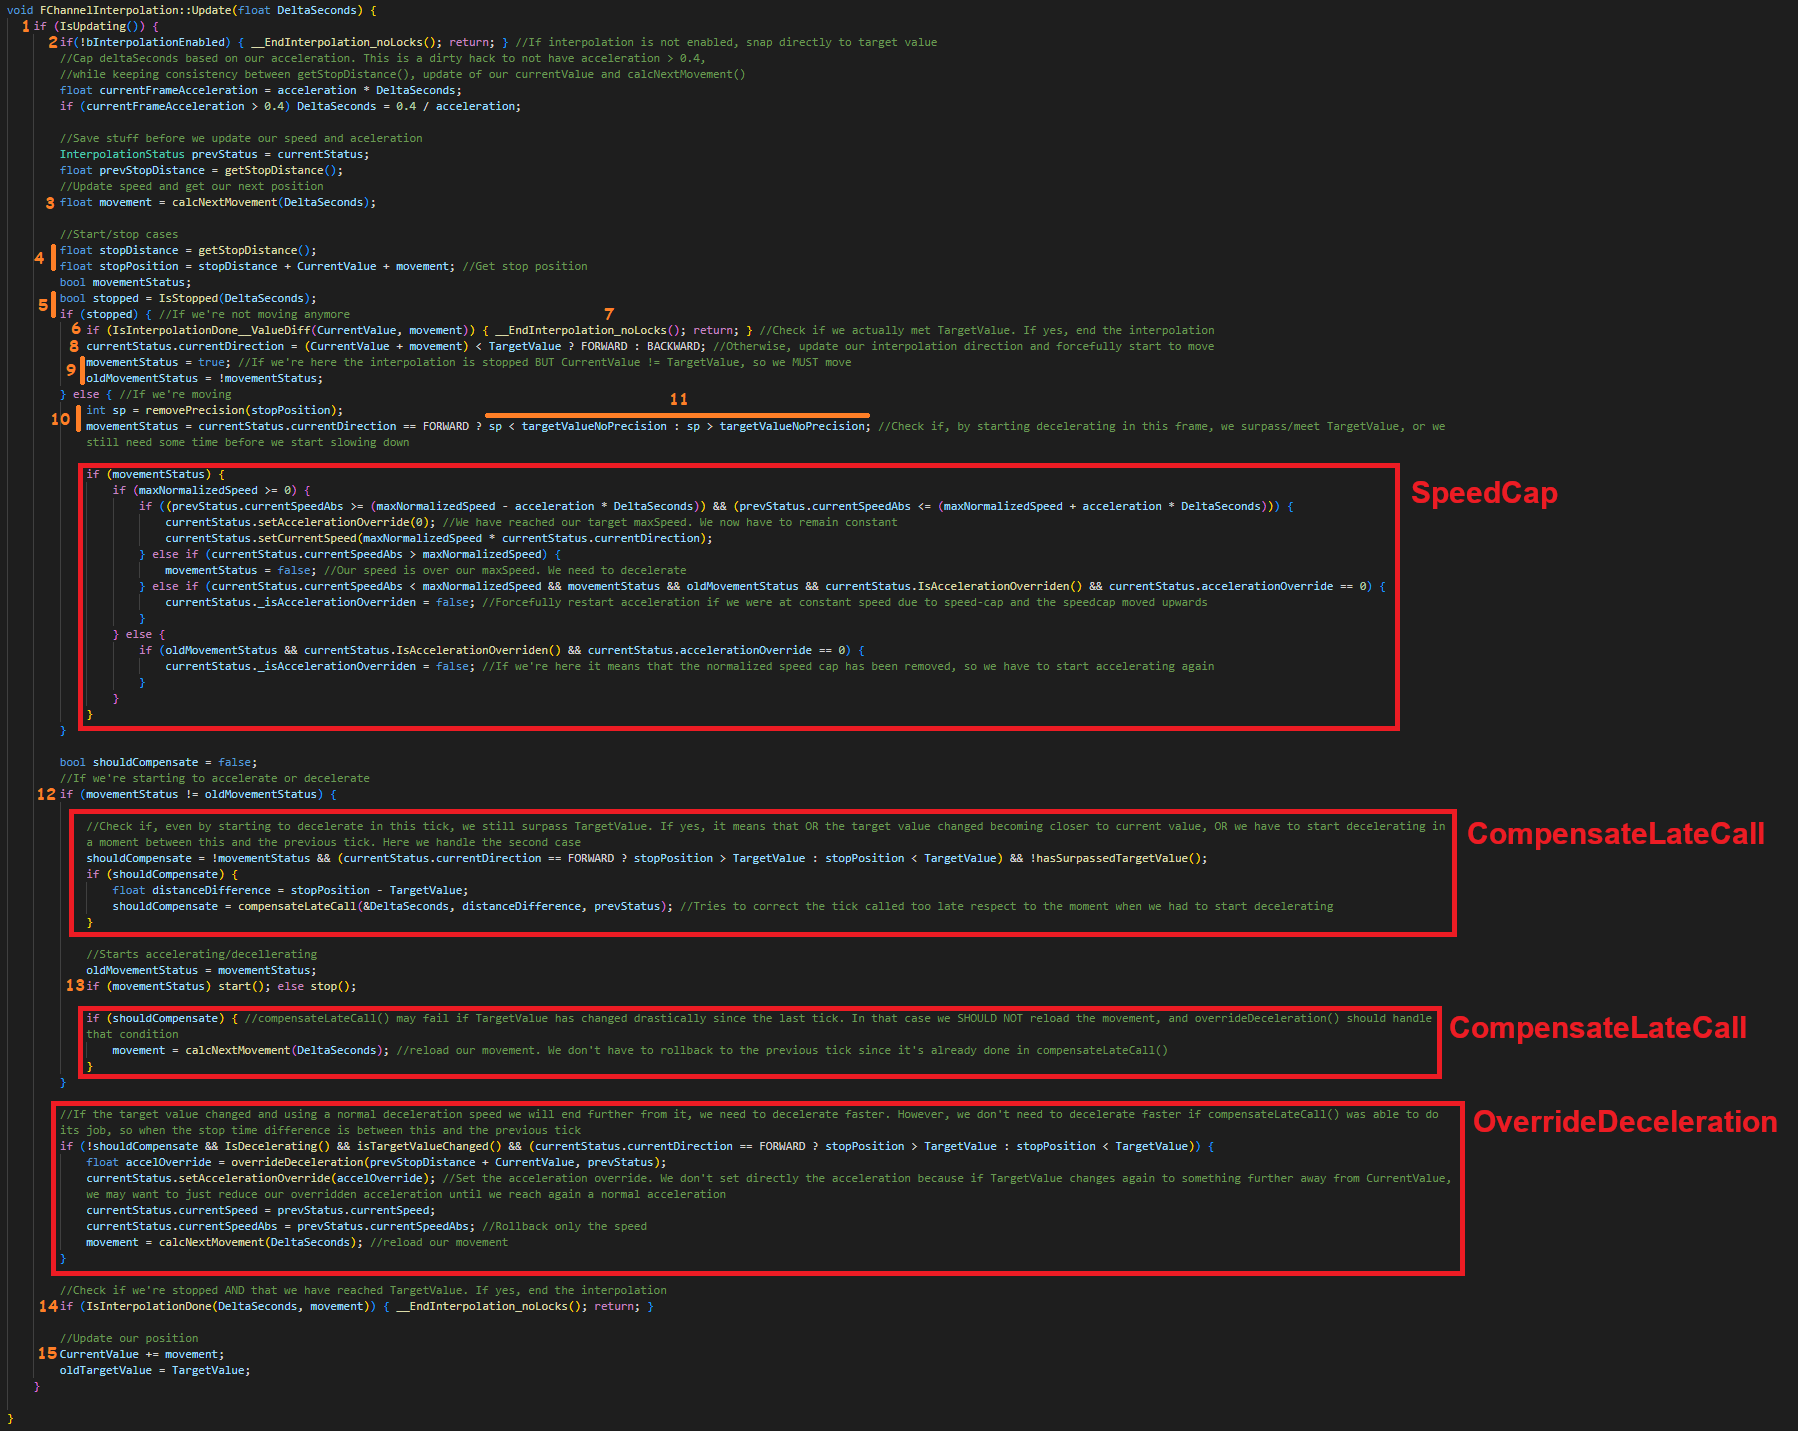
\includegraphics[width=1\linewidth]{img/interpolazione/Update.png}
    \caption{Funzione \lstinline{Update()}. In arancione i punti elencati nel capitolo \ref{subsec:4_trafficImplementation}, in rosso le nuove funzionalità.}
    \label{fig:4_Update}
\end{figure}
\begin{figure}[H]
    \centering
    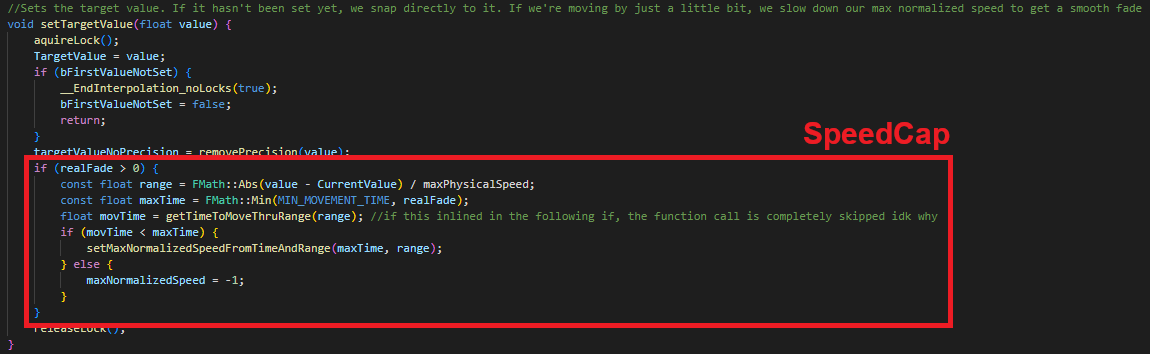
\includegraphics[width=1\linewidth]{img/interpolazione/SetTargetValue.png}
    \caption{Funzione \lstinline{SetTargetValue()} con l'aggiunta, in rosso, del codice per l'attivazione dello SpeedCap.}
    \label{fig:4_SetTargetValue}
\end{figure}

\end{document}